\section{Introduction}

\subsection{Background} \label{background}
Pharmaceutical research into drugs and their effects on human's often covers a wide range of areas, from analysis of the chemical attributes of the medication, to investigating the result of prescribing a variety of different drug regimens (for example how varying the time period or combinations certain drugs are given with can affect the outcomes for patients \cite{doi:10.1056/NEJMoa011954}). Part of this process of researching new drugs involves the characterisation of the pharmacokinetics and pharmacodynamics of the drug as part of the legal requirements for their authorisation for use inside the European market \cite{2001_83_EC_Directive_For_Pharmacokinetic_Characterisation}. The concepts of pharmacokinetics and pharmacodynamics are relatively simple to understand at a basic level. Pharmacokinetics is the study of the physical process of drug absorption, distribution, metabolism, and excretion, whereas pharmacodynamics is the body's biological response to a given drug. These are both typically modelled through the use of various chemical and mathematical analysis of the drug with the combination of the two being able to be thought of as a relationship between the level of exposure to a drug and the response the body has to it \cite{holford1982kinetics}. The reasoning behind this kind of analysis of new medication is related to figuring out the Therapeutic Window of the drug and ensuring that any new regimen maintains concentrations within this window. The Therapeutic Window is a period of concentrations between the Minimum Toxic Concentration (MTC) and the Minimum Effective Concentration (MEC) of the drug. The MTC of the drug is simply the minimum concentration of the drug which would be toxic to a person causing serious side effects, as such the aim is typically to ensure that concentrations are lower than this. On the other hand, the MEC of the drug is the minimum concentration at which the drug may be considered to be having the desired effect on the patient. The graph shown in Figure \ref{fig:theraputic_window} demonstrates how these are related to each other in terms of a typical drug adsorption profile. 
	
\begin{figure}[h]
	\centering
	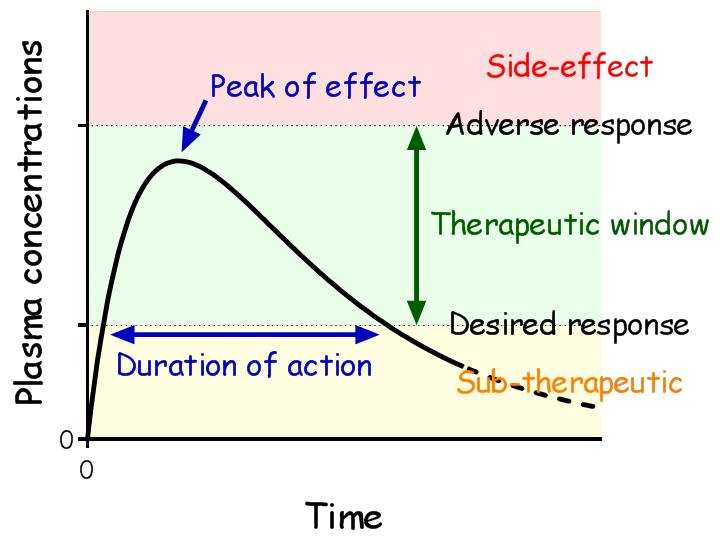
\includegraphics[width=0.7\textwidth]{Images/therapeutic-window.jpg}
	\caption{Plot showing Minimum Toxic Concentration, Minimum Effective Concentration and their relation to the Therapeutic Window \cite{Therapeutic_Index_And_Window}}
    \label{fig:theraputic_window}
\end{figure}

	
In terms of this project, the therapeutic window of many common chemotherapeutic drugs (such as cyclophosphamide) are typically very narrow \cite{cyclophosphamide_details}. As such, it is of high importance to ensure that all cumulative effects as a result of long term exposure to these medications are taken in to consideration when modelling the excretion and adsorption of them. This is especially true with respect to going above the MTC of drugs with therapeutic windows which are narrow as this can result in serious changes in the expected outcome for a patient \cite{Clinical_Pharmacokinetics_and_Pharmacodynamics_Concepts}.

As part of attempts to better characterise the non-linear effects which some drugs can cause after prolonged use, such as deep tissue trapping and long term accumulation, new approaches have recently been developed to aid in modelling these phenomenon \cite{ion_trapping, cumlative_effects}. To date, standard methods of modelling these systems have focused on the use of zero order and first order differential equations \cite{Clinical_Pharmacokinetics_and_Pharmacodynamics_Concepts} in conjunction with compartmental models to track the concentrations of a drug in different kinetically similar parts (or "compartments") of the body (although different compartments have no direct relationship anatomically) \cite{Compartmental_modeling_in_Pharmacokinetics}. These models however fail to take into account the non-linear elements of the model, and as such the recent research instead attempts to make use of a concept known as fractional-order calculus to model these systems. These fractional order pharmacokinetic systems have a number of benefits over the standard integer order systems. First and foremost is that fractional order pharmacokinetics allows non-linear elements to be taken into account in the model in stark contract to first and zero order systems. Secondly, the fact that fractional order pharmacokinetics, unlike first and zero order pharmacokinetics, take into account an entire weighted history of the system, means that when repeat maintenance doses are given to a patient, the impact of the "first-pass effect" and use of other techniques like a loading dose may be accounted for in calculations \cite{Clinical_Pharmacokinetics_and_Pharmacodynamics_Concepts}. 

\subsection{Objectives} \label{objectives}

Based on this background, this project has three elements to it. The first of these is to develop a fractional order model capable of simulating fractional order pharmacokinetics in a single compartment system. This will then be used to estimate the order and initial conditions of a given dataset using a least squares methodology. Following on from this, the project has been further developed using Bayesian statistics, through the provision of a set of prior distributions for the estimated parameters which when used help to produce results with higher credibility \cite{statistical_rethinking}. This finally culminates in a system which is capable of using live streamed data to perform the estimations, with new information allowing for updated estimations of noise in the system. 

This work has a number of benefits for industry in terms of its potential applications. In its current state this system will allow for further investigation into new methods of personalising medicine, with the parameters being estimated potentially being able to be used to design specific drug regimens for specific patients. This in turn may allow given fractional order values to be correlated, along with other pieces of patient information such as demographics and other pharmacokinetic parameters with patient outcomes, allowing more for informed decisions around patient treatment.

The developments in this field have not been possible in the past primarily as a result of the large amount of processing power required to perform the calculations when a large number of steps are estimated. Of course, in the last 30 years a variety of fields have been able to begin making use of Bayesian statistical methods and machine learning as a result rapid improvements in computational abilities.

This document therefore shall outline, over the course of the following pages, the theory, and further define the objectives, methodology and results of this project. These shall be analysed in the context of other research papers which shall be used to provide further insight into the current state of this area of enquiry. Additionally specific details of the software produced shall also be included in this document to act as documentation for any future progress that may occur with respect to this project.

\subsection{Current Literature} \label{current_literature}

To date there have been a selection of papers written which have approached the use of fractional order derivatives in the context of pharmacokinetics. One paper of interest is the International Federation of Automatic Control's \textit{Modeling and administration scheduling of fractional-order pharmacokinetic systems} \cite{Modeling_and_administration_scheduling}. The primary objective of this paper is to identify a numerical method for the simulation of a fractional order system and then to implement this such that the chosen method is used to simulate the pharmacokinetics of a given drug which is confirmed by means of a optimal control problem. 

In terms of the approach taken in this paper, a number of different forms of fractional order derivatives were reviewed. These included the Caputo $\gls{caputo_derivative}$, Riemann-Liouville $\gls{riemann_liouville_derivative}$ and the Gr\"{u}nwald-Letnikov $\gls{grunwald_letnikov_derivative}$ derivatives, which are operators used to form fractional-order differential equations. Upon addressing these and providing definitions the primary focus of the paper is then approached, looking at a variety of methods of solving Fractional order Differential Equations (FDE's) numerically (although it is pointed out that in some cases analytical solutions may exist) \cite{garrappa2015numerical}. 

Across this investigation three primary areas are focused on for solving FDE's: using the s-domain through integer order rational transfer functions approximations, numerical discretised approximations in the time domain, the inverse Laplace transformation solved numerically. The analysis of the different methods of solving an FDE resulted in a number of interesting conclusions that had an impact on the development of this project. For example, the conclusion that solving an FDE system using s-domain methods, whilst capable of providing a reasonably accurate solution, is not a reasonable proposition for a constrained system. This in conjunction with the information that the time domain approximation method highlighted in the paper, which involved the use of a discretised version of the Gr\"{u}nwald-Letnikov derivative, is less dependent on the step size for high precision and is more dependent on having a long history of points.

In addition to this, the next area this paper covered was to design a drug administration schedule using an optimal control problem. The problem as formulated in this paper has a point which should be noted for future consideration in a practical situation. It appears that the formulated cost function has the basic assumption that the parameters of the system are known in some capacity in advance (i.e. the order, initial conditions, etc are already available, thought they may not be precisely known). This is useful to know, given it highlights the novel nature of the work completed in this project, in addition to the fact it also demonstrates a clear use case for the work being completed in this project. 

Another paper which has been published and covers this area of academic work is that of the IFAC Proceedings Volumes, titled \textit{Controlled Drug Administration by a Fractional PID} \cite{Controlled_Drug_Administration}. This paper has the objectives of designing a fractional-order PID controller and evaluating its dynamics characteristics and ability to mitigate noise in the system. In the case of this paper, whereas in others mentioned, discretised forms of the fractional order Gr\"{u}nwald-Letnikov operator were highlighted and used in the process of the paper to highlight differences between solving in time domain and s-domain, this paper specifically utilises the Riemann-Liouville and Caputo operators approximately solved using the Oustaloup filter for the time domain and exactly solved in the frequency domain. 

The primary reasoning in this paper is that the use of fractional order dynamics in the design of the PID system will in of itself help stabilise the concentrations of the example drug used in the process of demonstrating the PID design. Over the course of the paper, it is clear that the use of fractional order dynamics is useful to this end, with high levels of closed loop and external noise rejection and high gain-margin both present in the results for this approach. This is of course demonstrating that the design is capable of acting to provide the necessary characteristics to model drugs that have fractional order dynamics.

Of course one point not covered again in this paper is how the parameters for the fractional order system may be known. It is presumed that the order, and other necessities are previously available to the designer of the PID. Obviously for new drugs this is not true, in addition to the idea that the assumption has been made that the order of the drug is a constant for all situations. This however may not be true, with the potential being present that the drug may act as a different order system depending on the patient (or even depending on the previous concentrations of the drug in a patients system). 
